\documentclass[a4paper,10pt]{article}
\usepackage[utf8]{inputenc}
\usepackage{caption}
\usepackage{subcaption}
\usepackage{graphicx}
\usepackage{float}
\usepackage{listings}
%opening
\title{ECE 231 Project 2}
\author{Lawrence Liu, David Zheng, Rohit Bhat}

\begin{document}

\maketitle


\section{Problem 1 (Polarization)}
\subsection{Part (a)}
$I(U_1, U_2; Y_1, Y_2) = \\
I(X_1, X_2; Y_1, Y_2)=$\qquad($U_1, U_2$ can be determined from $X_1, X_2$ and vice versa).\\
$H(X_1, X_2) -H(X_1, X_2|Y_1, Y_2)=\\ \\
H(X_1)-H(X_1|Y_1, Y_2) + H(X_2) - H(X_2|Y_1, Y_2)=$ \qquad ($X_1, X_2$ are indepedendent and $X_1, X_2$ are also conditionally independent given $Y_1, Y_2$)\\ \\
$H(X_1) - H(X_1|Y_1) + H(X_2) - H(X_2| Y_2)=$ \qquad ($X_1$ is conditionally independent from $Y_2$ given $Y_1$, and $X_2$ is conditionally independent from $Y_1$ given $Y_2$). \\ \\
$I(X_1; Y_1) + I(X_2; Y_2)$, as desired.\\ \\
We also have:\\
$I(U_1, U_2; Y_1, Y_2) = \\
H(U_1, U_2) - H(U_1, U_2 | Y_1, Y_2) = \\
H(U_1) + H(U_2) - H(U_1, U_2 | Y_1, Y_2)  = $\qquad($U_1, U_2$ are independent)\\
$H(U_1)+H(U_2) - H(U_1|Y_1, Y_2) - H(U_2 | Y_1, Y_2, U_1) = $\\
$H(U_1) - H(U_1|Y_1, Y_2)+H(U_2) - H(U_2 | Y_1, Y_2, U_1) = $\\
$I(U_1; Y_1, Y_2) + I(U_2; Y_1, Y_2, U_1)$, as desired.\\
\subsection{Part (b)}
Because $X_1, X_2$ go through identitical channels with identical capacities to become $Y_1, Y_2$, we must have $I(X_1; Y_1) = I(X_2; Y_2)$\\
To prove the right hand inequality:\\
$I(X_2; Y_2) =\\
H(X_2) - H(X_2 | Y_2) \leq\\
H(X_2) - H(X_2| Y_1, Y_2, U_1) =\\
I(X_2; Y_1, Y_2, U_1)= \\
I(U_2; Y_1, Y_2, U_1)$, as desired.\\
To prove the left hand inequality:\\
$I(U_1; Y_1, Y_2) = \\
I(U_1; Y_1, Y_2)=\\
I(U_1; Y_1 | Y_2) + I(U_1; Y_2)$\\
The second term is $0$ because $Y_2$ is independent from $U_1$.\\
We have:\\
$I(U_1; Y_1 | Y_2) = \\
I(X_1 \oplus X_2 ; Y_1|Y_2) \leq\\
I(X_1, X_2; Y_1 | Y_2)=$ \qquad (as $X_1, X_2$ uniquely determines $X_1 \oplus X_2$)\\
$I(X_1; Y_1 | Y_2) = $ \qquad ($X_2$ is independent from $X_1, Y_1$ even given $Y_2$)\\
$I(X_1; Y_1)$ \qquad ($Y_2$ is independent from $X_1, X_2$)\\
This is what we wanted to prove.
\section{Problem 2 (Polarization of BEC)}
Using the fact that $BEC(p)$ has capacity $1-p$, we have:\\
The capacity of $W^-$ is $1-2p + p^2 = (1-p)^2$\\
The capacity of $W$ is $1 - p$\\
The capacity of $W^+$ is $1 - p^2$\\
It is clear that $(1-p)^2 \leq 1 - p$ as $0 \leq 1-p \leq 1$. \\
It is also clear that $1-p \leq 1-p^2$ as $0 \leq p\leq 1$. \\
Therefore channel $W^-$ is worse than $W$, and $W^+$ is better than $W$.
\section*{Problem 3 (Coding Problem: Polarization of BEC)}
We get the following plots for $p=0.3$\\
\begin{figure}[H]
    \centering
    \begin{subfigure}{.5\textwidth}
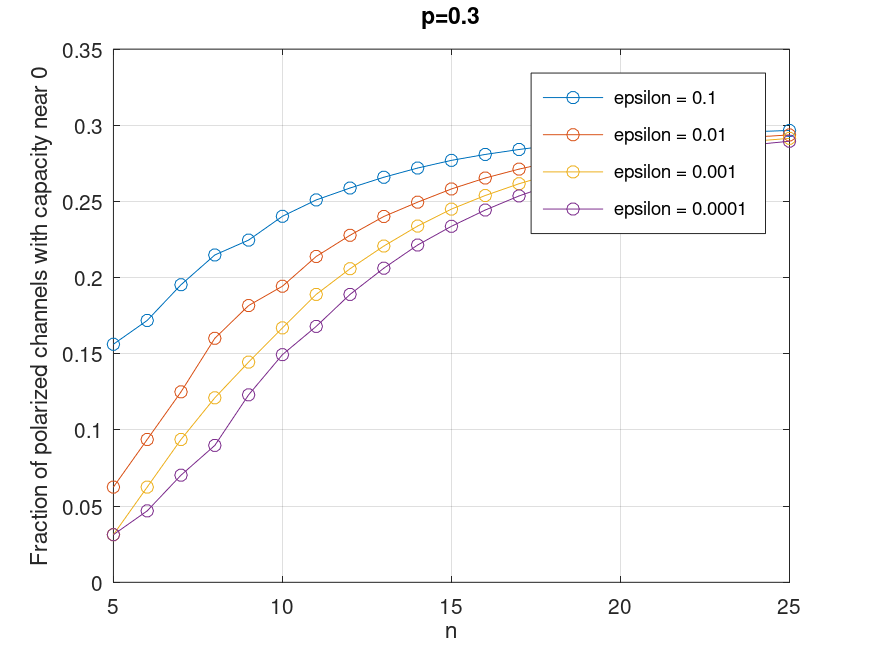
\includegraphics[width=.9\linewidth]{code/p=0.3 near 0.png}
    \end{subfigure}%
    \begin{subfigure}{.5\textwidth}
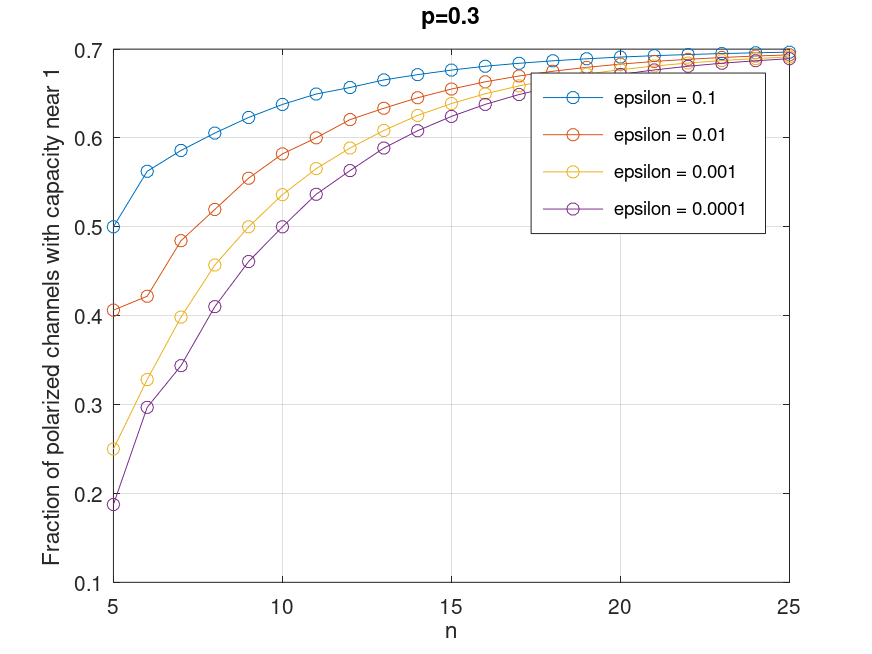
\includegraphics[width=.9\linewidth]{code/p=0.3 near 1.png}
    \end{subfigure}
\end{figure}
And the following plots for $p=0.6$\\
\begin{figure}[H]
    \centering
    \begin{subfigure}{.5\textwidth}
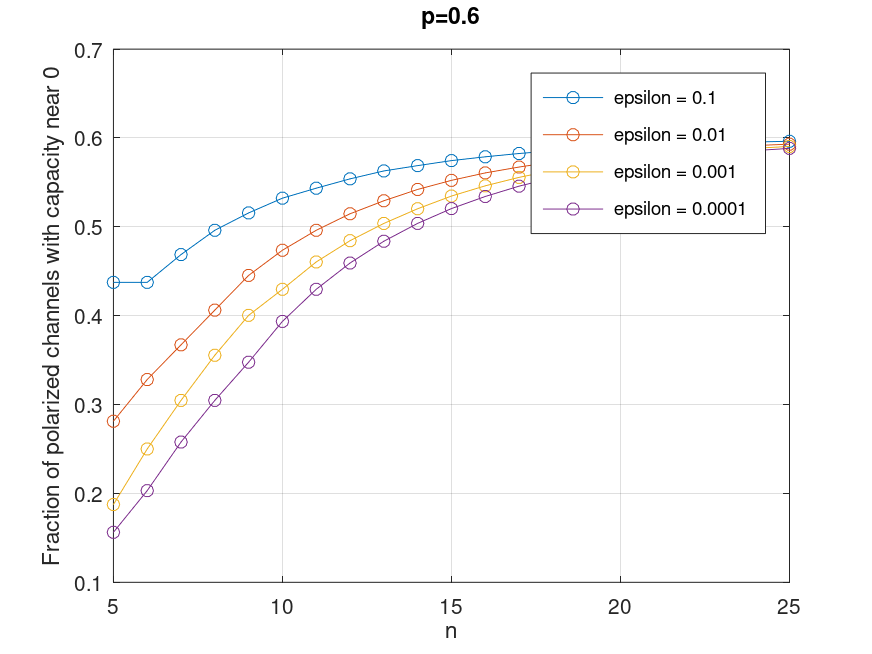
\includegraphics[width=.9\linewidth]{code/p=0.6 near 0.png}
    \end{subfigure}%
    \begin{subfigure}{.5\textwidth}
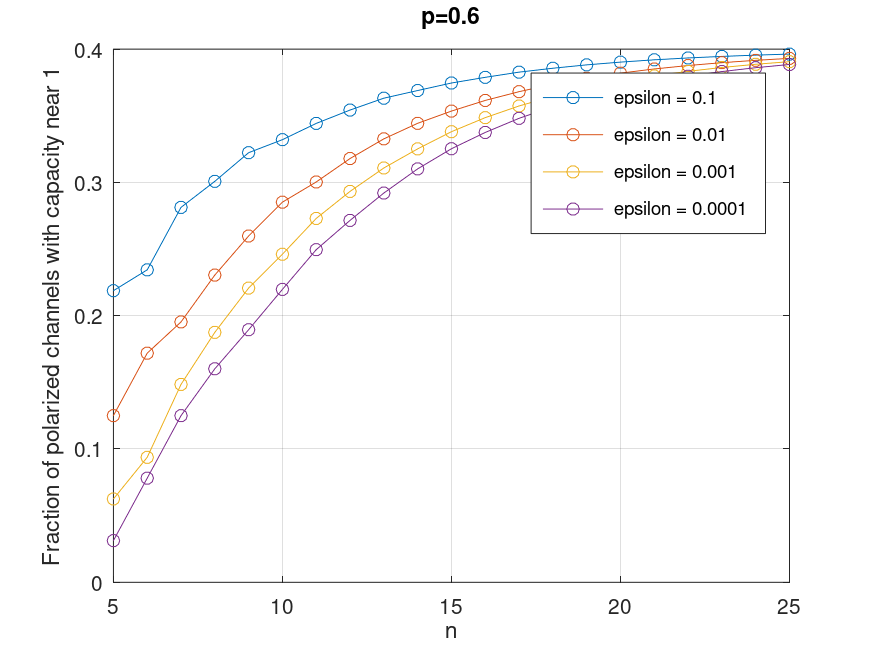
\includegraphics[width=.9\linewidth]{code/p=0.6 near 1.png}
    \end{subfigure}
\end{figure}
And the following plots for $p=0.8$\\
\begin{figure}[H]
    \centering
    \begin{subfigure}{.5\textwidth}
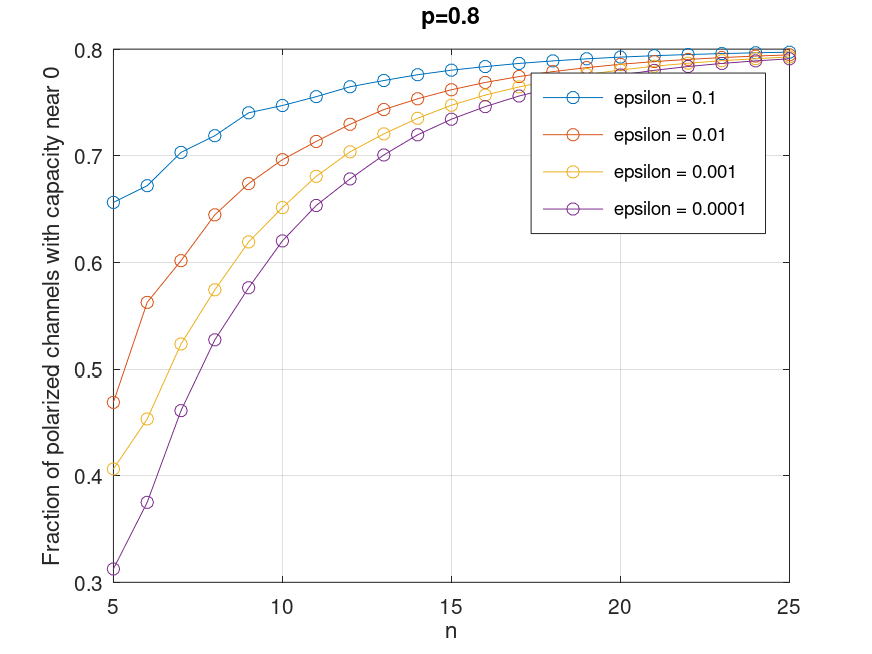
\includegraphics[width=.9\linewidth]{code/p=0.8 near 0.png}
    \end{subfigure}%
    \begin{subfigure}{.5\textwidth}
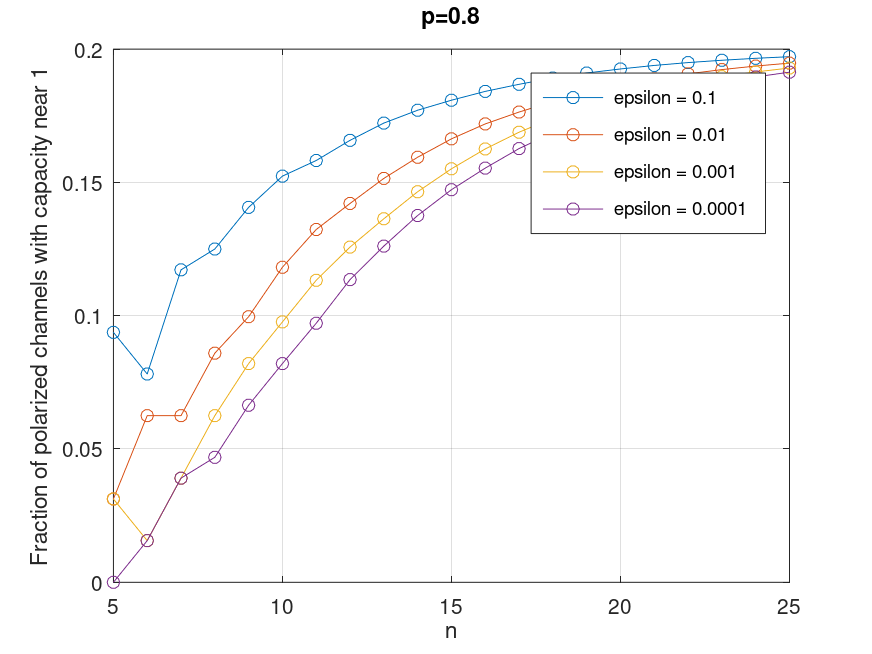
\includegraphics[width=.9\linewidth]{code/p=0.8 near 1.png}
    \end{subfigure}
\end{figure}
This was generated with the following code:\\
\lstinputlisting[language=Octave]{code/code_snippet_prob_3.m}
Note that because the plotting functions provided would only
plot for 1 value of p, I moved them inside the for loop. However because
we were instructed to not touch the code beyond the parts we could touch,
I left the original plotting functions in the code.
\section{Problem 4 (Using Polar codes for BPSK+AWGN channel)}
\subsection{(a)}
Using the formula for the capacity of the BPSK+AWGN channel found in 
the paper 
"Analysis and Design of Power-Efficient Coding Schemes With Parallel Concatenated Convolutional Codes"
by Simon Huettinger and J. Huber,
we have that the capcity is given by  
\begin{equation}
    C=1-\int_{-\infty}^{\infty} \frac{1}{\sqrt{2\pi\sigma^2}}e^{-\frac{(x-1)^2}{2\sigma^2}}\log_2(1+e^{-\frac{2x}{\sigma^2}})dx
\end{equation}
When we computed this integral we only did it from -20 to 20 since values
beyond that result in NaN values and thus results in an incorrect integral. The resulting
plot looks like\\
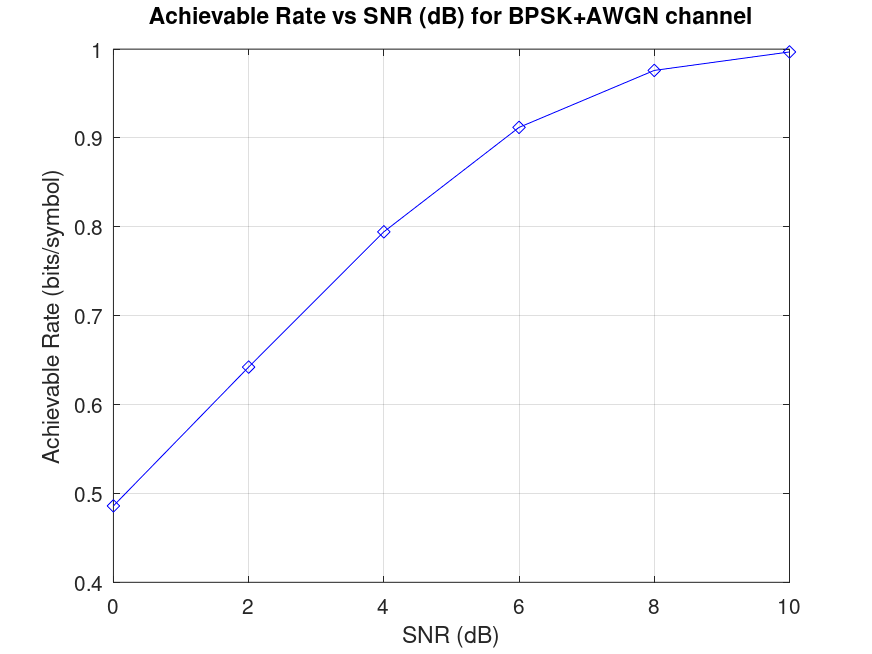
\includegraphics[scale=0.3]{code/Achievable Rate vs SNR (dB) for BPSK+AWGN channel.png}
\subsection{(b)}
We get the following plot for BER vs encoding rate for diffrerent SNR values\\
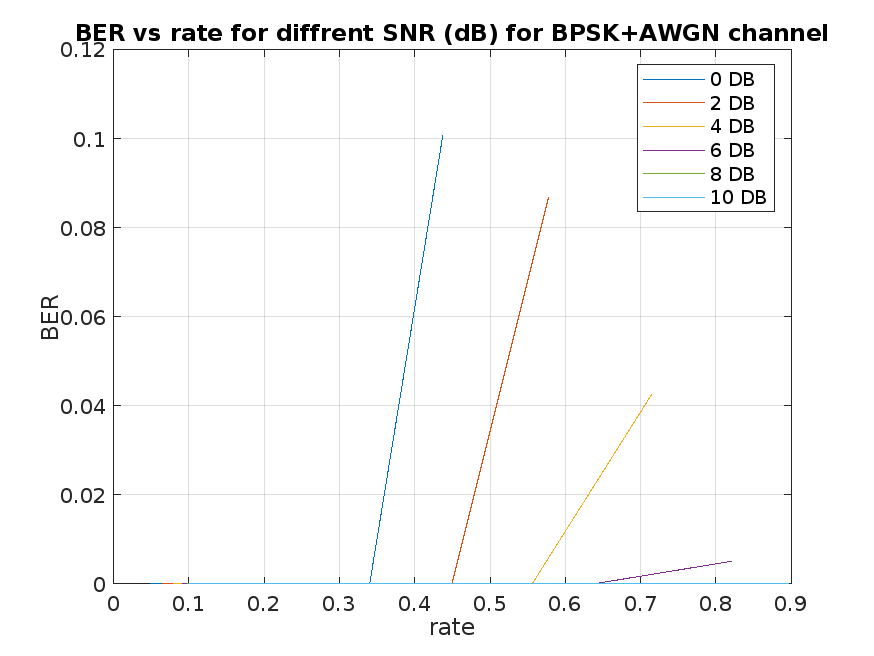
\includegraphics[scale=0.9]{code/BER vs rate for diffrent SNR (dB) for BPSK+AWGN channel.png}
\subsection{(c)}
We get the following plot for FER vs encoding rate for diffrerent SNR values\\
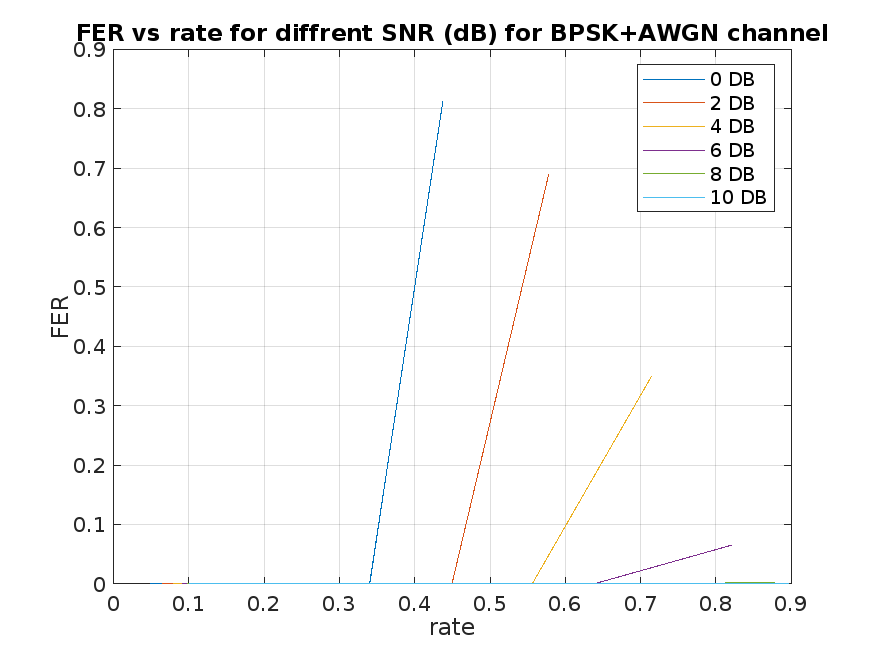
\includegraphics[scale=0.9]{code/FER vs rate for diffrent SNR (dB) for BPSK+AWGN channel.png}
\\\textit{note:} I modified the code outside of the comments saying to modify the code
to have a plotting function, and have the rates be iterated over as a for loop
nested inside a for loop for the SNR values. Also I reduced the number of trials
to make the code run faster. \\\\The code to do everything for
problem 4 is included below:
\lstinputlisting[language=Octave]{code/code_snippet_prob_4.m}
\section{How we divided up the work}
David and Rohit did problem 1 and 2, Lawrence did problem 3, and Lawrence 
and David did problem 4.
\end{document}